\documentclass[../sparc.tex]{subfiles}
\graphicspath{{\subfix{../images/}}}
\begin{document}

%%%%%%%%%%%%%%%%%%%%%%%%%%%%%%%%%%%%%%%%%%%%%%%%%%%%%%%%%%%%%%%%%%%%%%%%%%%%%%%%
\section{Реализация управления}

Для управления игровым персонажем нам потребуется некоторое устройство ввода
информации в наш компьютер (микроконтроллер).  Мы сделаем своё ``устройство
ввода'', состоящее из нескольких кнопок, расположенных на макетной плате.

\subsection{Подключение кнопки}

Попробуем подключить кнопку к Arduino.  Кнопка по своей сути не более чем
замыкатель двух контактов.  Самым простым аналогом кнопки являются два
разъединённых провода (разомкнутая электрическая цепь), которые можно соединить
между собой, или опять разъединить.  Само собой, такой способ управления
устройством неудобен (и даже небезопасен, при больших напряжениях и токах в
электрической цепи), поэтому кнопки обычно представлены некими закрытыми
устройствами, которые имеют некий способ замыкать цепь без необходимости брать в
руки концы проводов.

Кнопки по принципу работы бывают разные.  Самый простой их вид -- \emph{тактовые
кнопки}.

``Тактовыми'' называются кнопки, которые не ``запоминают'' своё состояние, и
сразу же после нажатия возвращаются в исходное состояние (как правило,
разомкнутое.)

Другой вид кнопок, с которыми мы сталкиваемся в быту -- это те, которые
``запоминают'' своё состояние; такие кнопки обычно называются
``переключателями''.

На рис. \ref{fig:game-dev-button-00} можно видеть один из возможных вариантов
подключения кнопки.  Можно подумать, что такой вариант достаточен -- когда
кнопка нажата, то цепь замыкатся и ток идёт от \texttt{5V} до цифрового порта
номер 2.  И действительно, в этом случае с порта можно считать значение 1
(\texttt{HIGH}).

\begin{figure}[ht]
  \centering
  \begin{circuitikz}
    \draw (3.5, 0) node[
      dipchip,
      num pins=2,
      external pins width=0.0,
      no topmark,
      hide numbers,
      xscale = 2.5,
      yscale = 2.5](C1){Arduino};
    \node [above left, font=\small] at (C1.bpin 1) {5V};
    \node [above right, font=\small] at (C1.bpin 2) {2};
    \draw
    (C1.bpin 1) to[short]
    (0, 0) to[short]
    (0, 4) to[push button, l=Тактовая кнопка] (7, 4)
    (7, 4) to[short]
    (7, 0) to[short]
    (C1.bpin 2);
  \end{circuitikz}
  \caption{Возможная схема подключения кнопки к Arduino.}
  \label{fig:game-dev-button-00}
\end{figure}

Пример простейшей программы, считывающей значение с кнопки, представлен ниже.

\begin{minted}{cpp}
  void setup() {
    pinMode(2, INPUT);
  }

  void loop() {
    // Считываем значение с кнопки и сохраняем в новую переменную "value".
    int value = digitalRead(2);
    // Далее эту переменную можно использовать в коде, чтобы определить
    // состояние кнопки: если в переменной находится значение 1,
    // то кнопка нажата, если 0 -- то не нажата.
  }
\end{minted}

Чтобы наглядно получить представление о том, как значение на кнопке будет
меняться при нажатии, мы можем дабавить вывод данных на компьютер.

\begin{minted}{cpp}
  void setup() {
    pinMode(2, INPUT);
    Serial.begin(9600);
  }

  void loop() {
    // Считываем значение с кнопки и сохраняем в новую переменную "value".
    int value = digitalRead(2);
    // Далее эту переменную можно использовать в коде, чтобы определить
    // состояние кнопки: если в переменной находится значение 1,
    // то кнопка нажата, если 0 -- то не нажата.

    // Выводим значение с кнопки в порт.
    Serial.println(value);
  }
\end{minted}

К сожалению, наблюдение за значенем на кнопке скорее всего нам покажет, что даже
когда кнопка не нажата, на ней иногда ``проскакивает'' значение 1.  Как такое
может быть?  Объяснение простое -- как мы видели в главе ``Белый шум'', вокруг
нас присутствует электромагнитный фон, который улавливается схемами и приводит к
тому, что иногда значение на цифровых портах переходит рубеж, после которого
Arduino считает это значение единицей.

Решить эту проблему можно как минимум двумя способами.  Первый способ
заключается в том, чтобы поставить специальный \emph{подтягивающий резистор},
который будет подтягивать значение на порту, куда подключена кнопка, к земле
(GND.)

\begin{figure}[ht]
  \centering
  \begin{circuitikz}
    \draw (3.5, 0) node[
      dipchip,
      num pins=3,
      external pins width=0.0,
      no topmark,
      hide numbers,
      xscale = 2.5,
      yscale = 2.5](C1){Arduino};
    \node [above left, font=\small] at (C1.bpin 1) {5V};
    \node [above right, font=\small] at (C1.bpin 2) {2};
    \node [above right, font=\small] at (C1.bpin 3) {GND};
    \draw
    (C1.bpin 1) to[short]
    (0, 0.35) to[short]
    (0, 4) to[push button, l=Тактовая кнопка] (9, 4)
    (9, 4) to[short]
    (9, -0.35) to[short]
    (C1.bpin 2);
    \draw
    (C1.bpin 3) to [short]
    (7, 1) to [european resistor, l=$R_1$]
    (8, 1) to [short]
    (9, 1);
    
  \end{circuitikz}
  \caption{Схема подключения кнопки к Arduino с подтягивающим резистором.}
  \label{fig:game-dev-button-with-pull-down-resistor}
\end{figure}

Второй способ подключения кнопки -- использование встроенного в Arduino
подтягивающего резистора, который подключен на 5V.  В этом случае схема
подключения значительно упрощается и становится похожа на то, что было показано
на рис. \ref{fig:game-dev-button-00}, но с одним отличием: цифровой порт должен
при нажатии на кнопку замыкаться не на \texttt{5V}, а на \texttt{GND}
(см. рис. \ref{fig:game-dev-button-with-pull-up-resistor}.)

\begin{figure}[ht]
  \centering
  \begin{circuitikz}
    \draw (3.5, 0) node[
      dipchip,
      num pins=2,
      external pins width=0.0,
      no topmark,
      hide numbers,
      xscale = 2.5,
      yscale = 2.5](C1){Arduino};
    \node [above left, font=\small] at (C1.bpin 1) {GND};
    \node [above right, font=\small] at (C1.bpin 2) {2};
    \draw
    (C1.bpin 1) to[short]
    (0, 0) to[short]
    (0, 4) to[push button, l=Тактовая кнопка] (7, 4)
    (7, 4) to[short]
    (7, 0) to[short]
    (C1.bpin 2);
  \end{circuitikz}
  \caption{Схема подключения кнопки к Arduino при использовании встроенного
    подтягивающего резистора к 5V.}
  \label{fig:game-dev-button-with-pull-up-resistor}
\end{figure}

Настройка порта в этом случае должна производиться на режим
\texttt{INPUT\_PULLUP}.  В остальном же код нашего примера остаётся без
изменений.

\begin{minted}{cpp}
  void setup() {
    pinMode(2, INPUT_PULLUP);
    Serial.begin(9600);
  }

  void loop() {
    // Считываем значение с кнопки и сохраняем в новую переменную "value".
    int value = digitalRead(2);
    // Далее эту переменную можно использовать в коде, чтобы определить
    // состояние кнопки: если в переменной находится значение 1,
    // то кнопка нажата, если 0 -- то не нажата.

    // Выводим значение с кнопки в порт.
    Serial.println(value);
  }
\end{minted}

При таком использовании работа с кнопкой ``инвертируется'' -- когда она нажата,
то значение на порту будет ``0'' (\texttt{LOW}), а когда не нажата, то ``1''
(\texttt{HIGH}.)

\subsection{Обработка нажатий}

Для начала зададим номер порта, куда подключена наша (пока единственная) кнопка,
в виде именованной константы \texttt{BUTTON\_R} (``R'' от слова ``Right'',
``Вправо''.)

\begin{minted}{cpp}
  #include <LiquidCrystal_I2C.h>

  LiquidCrystal_I2C lcd(0x27,  16, 2);

  // Кнопки управления.
  const char BUTTON_R = 2;      // Кнопка ``Вправо''

  const char PLAYER = '@';

  int player_x = 0;
  int player_y = 0;
\end{minted}

Далее в \texttt{setup} необходимо настроить режим работы порта для кнопки через
\texttt{pinMode}, как мы делали это в предыдущих примерах.

\begin{minted}{cpp}
  void setup() {
    lcd.init();
    lcd.backlight();

    // Настройка кнопок управления.
    pinMode(BUTTON_R, INPUT_PULLUP);
  }
\end{minted}

После этого следует определиться, как мы будем обрабатывать нажатия кнопок.
Сейчас самым простым для нас способом обработки нажатий является поочерёдный
опрос кнопок, про другие способы мы с вами поговорим позднее.

Для обработки нажатий мы будем в \texttt{loop} проверять значение на порту, куда
подключена кнопка, используя уже знакомый нам \texttt{digitalRead}, и если
значение будет \texttt{LOW}, то менять позицию персонажа.

\begin{minted}{cpp}
  void loop() {
    if (digitalRead(BUTTON_R) == LOW) {
      player_x++;
    }
    lcd.setCursor(player_x, player_y);
    lcd.print(PLAYER);
  }
\end{minted}

Таким образом, при нажатии кнопки ``ВПРАВО'' мы будем получать смещение
персонажа вправо.

В общем виде, код нашей игры на текущий момент выглядит так:

\begin{minted}{cpp}
  #include <LiquidCrystal_I2C.h>

  LiquidCrystal_I2C lcd(0x27,  16, 2);

  // Кнопки управления.
  const char BUTTON_R = 2;      // Кнопка ``Вправо''

  const char PLAYER = '@';

  int player_x = 0;
  int player_y = 0;

  void setup() {
    lcd.init();
    lcd.backlight();

    // Настройка кнопок управления.
    pinMode(BUTTON_R, INPUT_PULLUP);
  }

  void loop() {
    if (digitalRead(BUTTON_R) == LOW) {
      player_x++;
    }
    lcd.setCursor(player_x, player_y);
    lcd.print(PLAYER);
  }
\end{minted}

Здесь однако же кроется проблема -- при единичном (на наш взгляд) нажатии
кнопки, игрок может пробежать до конца карты, или даже скрыться за её пределами.
Это возникает, так как короткое (единичное) нажатие на кнопку с точки зрения
человека занимает огромное время с точки зрения компьютера.  За то время, пока
мы держим палец на кнопке, перед тем, как её отпустить, функция \texttt{loop}
успевает сработать несколько раз; следовательно, несколько раз будет считано и обработано состояние кнопки.

Для борьбы с этой проблемой необходимо добавить короткую задержку (например, в
100мс) в конце \texttt{loop}:

\begin{minted}{cpp}
  void loop() {
    if (digitalRead(BUTTON_R) == LOW) {
      player_x++;
    }
    lcd.setCursor(player_x, player_y);
    lcd.print(PLAYER);

    // Задержка, чтобы избежать слишком быстрого считывания
    // нажатий на кнопки.
    delay(100);
  }
\end{minted}


Точно таким же образом мы можем добавить кнопку движения влево, слегка дополнив
код нашего примера.  Поскольку исходный код нашей игры будет дальше расти, для
краткости будем сокращать уже написанные части, акцентрируя внимание на том, что
поменялось.

\begin{minted}{cpp}
  // ... Код подключения библиотеки и создания
  //     переменной "lcd". ...

  // Кнопки управления.
  const char BUTTON_R = 2;      // Кнопка "Вправо"
  const char BUTTON_L = 3;      // Кнопка "Влево"

  const char PLAYER = '@';

  // ... Код задания переменных позиции игрока. ...

  void setup() {
    // ... Код настройки дисплея. ...

    // Настройка кнопок управления.
    pinMode(BUTTON_R, INPUT_PULLUP);
    pinMode(BUTTON_L, INPUT_PULLUP);
  }

  void loop() {
    if (digitalRead(BUTTON_R) == LOW) {
      player_x++;
    }
    if (digitalRead(BUTTON_L) == LOW) {
      player_x--;
    }
    lcd.setCursor(player_x, player_y);
    lcd.print(PLAYER);

    // Задержка, чтобы избежать слишком быстрого считывания
    // нажатий на кнопки.
    delay(100);
  }
\end{minted}

Запустите эту программу, попробуйте походить влево-вправо.  В скором времени вы
заметите, что есть серьёзная проблема -- игрок может выйти за пределы дисплея
(``уйти за карту''.)

\subsection{Ограничение движения игрока}
\index{Условия}

Чтобы исправить вышеописанную проблему, необходимо добавить проверки позиции
игрока прежде, чем позволить ему сдвинуться влево или вправо.  Эти проверки
нужны при обработке нажатий кнопок.

Для движения вправо нам нужно смотреть, не выйдет ли игрок при следуюем ``шаге''
(перемещении на клетку) за карту.  Поскольку мы знаем, что размер нашего дисплея
-- 16 столбцов, то мы можем ограничить движение вправо 15-й клеткой.

\begin{minted}{cpp}
  // ... Код, который мы писали до этого ...

  void loop() {
    if (digitalRead(BUTTON_R) == LOW) {
      // Делаем ограничение движения игрока вправо.
      // Если игрок уже на 15-й клетке, то дальше двигаться
      // ему нельзя.
      if (player_x < 15) {
        player_x++;
      }
    }
    if (digitalRead(BUTTON_L) == LOW) {
      player_x--;
    }
    lcd.setCursor(player_x, player_y);
    lcd.print(PLAYER);

    // Задержка, чтобы избежать слишком быстрого считывания
    // нажатий на кнопки.
    delay(100);
  }
\end{minted}

С движением влево нужна подобная же проверка, с разницей в том, что крайняя
левая точка у нас -- это нулевая клетка.

\begin{minted}{cpp}
  // ... Код, который мы писали до этого ...

  void loop() {
    if (digitalRead(BUTTON_R) == LOW) {
      // Делаем ограничение движения игрока вправо.
      // Если игрок уже на 15-й клетке, то дальше двигаться
      // ему нельзя.
      if (player_x < 15) {
        player_x++;
      }
    }
    if (digitalRead(BUTTON_L) == LOW) {
      // Делаем ограничение движения игрока влево.
      // Если игрок уже на нулевой клетке, то левее
      // двигаться ему уже некуда.
      if (player_x > 0) {
        player_x--;
      }
    }
    lcd.setCursor(player_x, player_y);
    lcd.print(PLAYER);

    // Задержка, чтобы избежать слишком быстрого считывания
    // нажатий на кнопки.
    delay(100);
  }
\end{minted}

Таким образом мы обработали оба случая, когда игрок мог выйти за нашу игровую
карту.

\subsection{Добавление объектов на карту}
\index{Двумерные массивы}

В играх вокруг игрока обычно разворачивается некоторое действие -- не-игровые
персонажи (Non-Playable Characters, сокращённо ``NPC'') ревностно патрулируют
территорию карты; появляются и исчезают различные объекты, с которыми можно
взаимодействовать; накоец, повсюду располагаются различные \emph{статические}
объекты, которые могут преграждать путь игроку, или же являться просто
элементами декора.

Простым способом расположить отдельный объект на карте является задание ему
координат на карте и отрисовка -- так же, как мы делаем это с игровым
персонажем.  Однако при создании двух переменных (для координаты по оси X и по
оси Y) на каждый объект, количество переменных будет расти очень быстро.  Только
представьте, что карта размером 20х4 может потенциально хранить 80 объектов, что
даёт суммарно 160 переменных для адресации каждого из них!  Для решения этой
проблемы мы должны прибегнуть к уже известным нам массивам, с одной оговоркой --
мы должны будем использовать \emph{двумерные массивы}.

Схематическое изображение двумерного массива можно увидеть на
рис. \ref{fig:2d-array-example}.

\begin{figure}[ht]
  \centering
  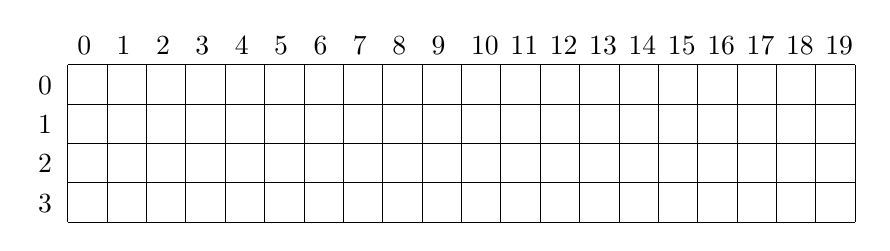
\begin{tikzpicture}
    \draw[step=0.5cm,black,very thin] (-5, -2) grid (5, 0);
    \foreach[count=\n from 0] \x in {-5, -4.5, ..., 4.5} {
      \draw (\x cm, 0) node[anchor=south west] {$\n$};
    }
    \foreach[count=\n from 0] \y in {-0.5, -1.0, ..., -2} {
      \draw (-5.5, \y) node[anchor=south west] {$\n$};
    }
  \end{tikzpicture}
  \caption{Схематическое изображение массива 4x20 (4 строки, 20 столбцов.)}
  \label{fig:2d-array-example}
\end{figure}

Можно также представить двумерный массив 4x20, как одномерный массив из 4-х
элементов, каждая ячейка которого содержит ссылку на ещё один одномерный массив
длиной 20 ячеек, как показано на
рис. \ref{fig:2d-array-example-with-references}.

\begin{figure}[ht]
  \centering
  \begin{tikzpicture}
    \draw[step=0.5cm,black,very thin] (-5, -2) grid (-4.5, 0);
    \draw[step=0.5cm,black,very thin] (-4, -2) grid (6, 0);
    \foreach[count=\n from 0] \x in {-4, -3.5, ..., 5.5} {
      \draw (\x cm, 0) node[anchor=south west] {$\n$};
    }
    \foreach[count=\n from 0] \y in {-0.5, -1.0, ..., -2} {
      \draw (-5.5, \y) node[anchor=south west] {$\n$};
    }
    \foreach[count=\n from 0] \y in {-0.25, -0.75, ..., -2} {
      \draw[{Circle}-{Stealth}]  (-4.8, \y) -- (-4, \y);
    }
  \end{tikzpicture}
  \caption{Схематическое представление массива 4x20 в виде одномерного массива
    из 4-х элементов со ссылками на одномерные массивы по 20 элементов.}
  \label{fig:2d-array-example-with-references}
\end{figure}

Для наших задач реализации игры нам потребуется задать массив, хранящий тип
данных \texttt{char}.

\end{document}
